\chapter{Sperimentazione della propagazione del suono}
\label{chap:sperimentazione_propagazione}

Il percorso metodologico delineato nel \autoref{chap:stato_arte} è stato tradotto in una campagna di misurazioni svolta in un corridoio di servizio situato a circa cinque metri sotto terra, largo \SI{1.2}{\meter}, lungo \SI{15}{\meter} e chiuso da una parete cieca, con una porta sul lato sinistro posta a \SI{10}{\meter} dall'origine che introduce nella camera laterale raffigurata in \autoref{fig:planimetria_tunnel}; la deviazione a novanta gradi corrisponde all'accesso a questa stanza, mentre il tunnel principale resta rettilineo fino al muro finale.\ La prova ha impiegato il dispositivo sperimentale sviluppato nella tesi, basato sulla piattaforma ESP32, sullo stadio di pilotaggio e sul trasduttore audio integrati \cite{Espressif2024,esp32techref,adafruit-guide}, programmato con il protocollo definito nella parte di implementazione software \cite{QuadraticInterpolationSpectralPeaks}.\ Il generatore ha riprodotto in sequenza tutte le frequenze previste dal protocollo, da \SI{1000}{\hertz} a \SI{9000}{\hertz} con passi di \SI{400}{\hertz}, mantenendo per ciascuna un livello in emissione di circa \SI{70}{\decibel_{SPL}} misurato all'ingresso del tunnel.\ Le misure di attenuazione sono state raccolte con il \textbf{Fonometro Tadeto}, dal costo di circa quindici euro, posato accanto alla scheda ricevente equipaggiata con l'implementazione software di decodifica, così da correlare in tempo reale la variazione del livello sonoro con la percentuale di pacchetti persi al crescere della distanza; i valori registrati alimentano le curve di \autoref{fig:profilo_db}.

All'ingresso del tunnel il segnale manteneva i \SI{70}{\decibel_{SPL}}, mentre a \SI{5}{\meter} lungo il tratto rettilineo il livello medio scendeva a \SI{65}{\decibel_{SPL}} e a \SI{10}{\meter} si attestava su \SI{62}{\decibel_{SPL}}; il valore minimo registrato contro la parete terminale dopo \SI{15}{\meter} è stato di \SI{55}{\decibel_{SPL}}, confermando una perdita complessiva di circa \SI{15}{\decibel}.\ Attraversando la porta sinistra, lasciata completamente aperta, l'operatore ha seguito il percorso spezzato verso la camera larga \SI{4}{\meter} e lunga \SI{3}{\meter}. A \SI{1.5}{\meter} dal varco la misura rimaneva su \SI{59}{\decibel_{SPL}}, ma collocandosi a \SI{3}{\meter} lungo la direzione principale della stanza si è osservato il crollo atteso a \SI{52}{\decibel_{SPL}}, seguito da un ulteriore assestamento a \SI{51}{\decibel_{SPL}} vicino alla parete opposta.\ La combinazione dei livelli e della presenza di superfici riflettenti ha comportato un comportamento frequenziale regolare: le componenti tra \SI{5}{\kilo\hertz} e \SI{7.4}{\kilo\hertz} hanno mostrato attenuazioni leggermente più pronunciate rispetto alle frequenze basse, ma sempre inferiori a \SI{2}{\decibel} di differenza rispetto al valore medio, preservando la leggibilità delle portanti in tutte le bande testate.\ Il rumore di fondo dell'ambiente sotterraneo è rimasto stabile su \SI{35}{\decibel_{SPL}}, garantendo quindi un margine superiore a \SI{16}{\decibel} anche nel punto più critico dopo la curva e permettendo alla catena ricevente di distinguere con chiarezza i pacchetti trasmessi.\ Le analisi sul traffico confermano che il percorso rettilineo ha mantenuto un tasso di perdita inferiore al \SI{5}{\percent} fino alla parete finale, mentre nella camera laterale l'incremento di attenuazione dopo i \SI{3}{\meter} dalla curva ha fatto salire la packet loss fino a circa \SI{18}{\percent}; le due serie sono riportate dalle linee verdi e arancioni di \autoref{fig:profilo_db} e hanno guidato la scelta di soglie conservative per l'allarme di riconnessione del protocollo.\ In una produzione reale, come evidenziato nell'analisi del \autoref{chap:stato_arte}, l'alimentazione a \SI{3.3}{\volt} verrebbe sostituita da uno stadio a rete intorno ai \SI{220}{\volt}, con un incremento di livello pari a $20\log_{10}\!\left(\tfrac{220}{3.3}\right) \approx \SI{36.5}{\decibel}$: l'emissione iniziale arriverebbe quindi a circa \SI{106.5}{\decibel_{SPL}} e, mantenendo invariata l'attenuazione osservata, porterebbe i livelli lungo il corridoio a \SI{101.5}{\decibel_{SPL}} dopo \SI{5}{\meter}, \SI{98.5}{\decibel_{SPL}} in prossimità della porta e \SI{91.5}{\decibel_{SPL}} contro il muro; nel ramo laterale si stimerebbero \SI{95}{\decibel_{SPL}} tre metri oltre la curva, valori che resterebbero nettamente separati dal rumore di fondo.

\begin{figure}[H]
    \centering
    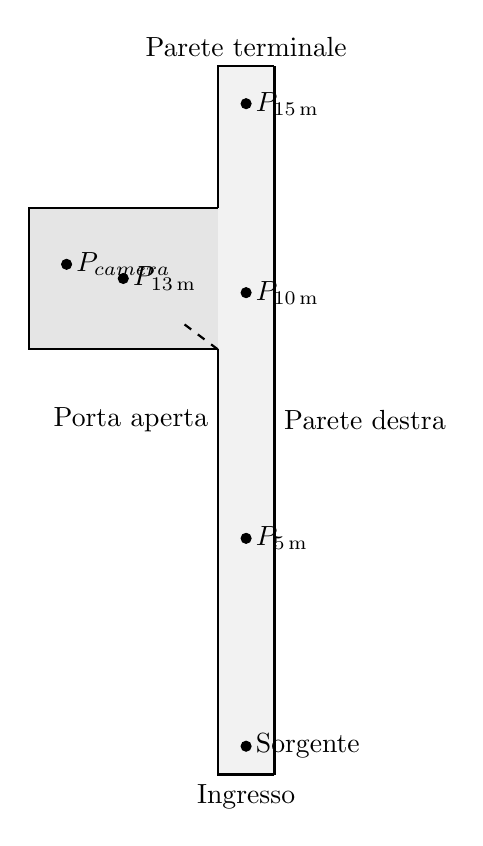
\begin{tikzpicture}[scale=0.6]
        \fill[gray!10] (-1.2,0) rectangle (0,15);
        \fill[gray!20] (-5.2,9) rectangle (-1.2,12);
        \draw[thick] (0,0) -- (-1.2,0) -- (-1.2,9);
        \draw[thick] (0,0) -- (0,15);
        \draw[thick] (0,15) -- (-1.2,15) -- (-1.2,12);
        \draw[thick] (-1.2,9) -- (-5.2,9) -- (-5.2,12) -- (-1.2,12);
        \draw[thick, dashed] (-1.2,9) -- (-2,9.6);
        \node[anchor=north] at (-0.6,0) {Ingresso};
        \node[anchor=south] at (-0.6,15) {Parete terminale};
        \node[anchor=west] at (0,7.5) {Parete destra};
        \node[anchor=east] at (-1.2,7.5) {Porta aperta};
        \filldraw[black] (-0.6,0.6) circle (3pt) node[anchor=west] {Sorgente};
        \filldraw[black] (-0.6,5) circle (3pt) node[anchor=west] {$P_{5\,\mathrm{m}}$};
        \filldraw[black] (-0.6,10.2) circle (3pt) node[anchor=west] {$P_{10\,\mathrm{m}}$};
        \filldraw[black] (-0.6,14.2) circle (3pt) node[anchor=west] {$P_{15\,\mathrm{m}}$};
        \filldraw[black] (-3.2,10.5) circle (3pt) node[anchor=west] {$P_{13\,\mathrm{m}}$};
        \filldraw[black] (-4.4,10.8) circle (3pt) node[anchor=west] {$P_{\text{camera}}$};
    \end{tikzpicture}
    \caption{Planimetria schematica del corridoio sotterraneo con indicazione dei punti di misura. La porta sul lato sinistro è stata mantenuta aperta durante la prova e consente l'accesso alla camera laterale.}
    \label{fig:planimetria_tunnel}
\end{figure}

\begin{figure}[H]
    \centering
    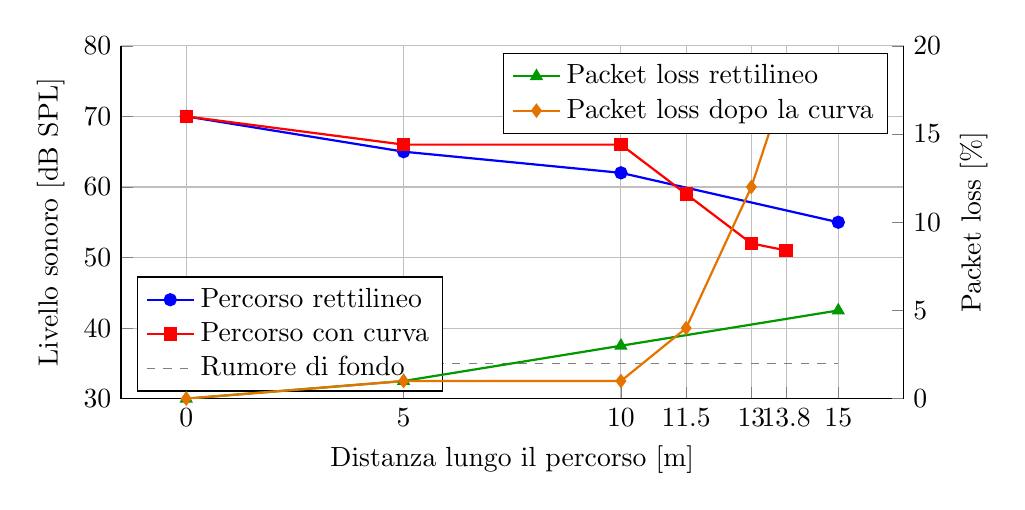
\begin{tikzpicture}
        \begin{axis}[
            name=audio,
            width=0.95\textwidth,
            height=0.5\textwidth,
            grid=both,
            axis y line*=left,
            axis x line*=bottom,
            xlabel={Distanza lungo il percorso [m]},
            ylabel={Livello sonoro [dB SPL]},
            ymin=30,
            ymax=80,
            xtick={0,5,10,11.5,13,13.8,15},
            ytick={30,40,50,60,70,80},
            legend style={at={(0.02,0.02)},anchor=south west},
            legend cell align=left
        ]
            \addplot[thick, color=blue, mark=*] coordinates {
                (0,70)
                (5,65)
                (10,62)
                (15,55)
            };
            \addlegendentry{Percorso rettilineo}
            \addplot[thick, color=red, mark=square*] coordinates {
                (0,70)
                (5,66)
                (10,66)
                (11.5,59)
                (13,52)
                (13.8,51)
            };
            \addlegendentry{Percorso con curva}
            \addplot[dashed, color=gray] coordinates {
                (0,35)
                (15,35)
            };
            \addlegendentry{Rumore di fondo}
        \end{axis}
        \begin{axis}[
            at={(audio.south west)},
            anchor=south west,
            width=0.95\textwidth,
            height=0.5\textwidth,
            axis y line*=right,
            axis x line=none,
            ymin=0,
            ymax=20,
            ytick={0,5,10,15,20},
            ylabel={Packet loss [\%]},
            legend style={at={(0.98,0.98)},anchor=north east},
            legend cell align=left
        ]
            \addplot[thick, color=green!60!black, mark=triangle*] coordinates {
                (0,0)
                (5,1)
                (10,3)
                (15,5)
            };
            \addlegendentry{Packet loss rettilineo}
            \addplot[thick, color=orange!90!black, mark=diamond*] coordinates {
                (0,0)
                (5,1)
                (10,1)
                (11.5,4)
                (13,12)
                (13.8,18)
            };
            \addlegendentry{Packet loss dopo la curva}
        \end{axis}
    \end{tikzpicture}
    \caption{Andamento medio dei livelli sonori misurati lungo il corridoio e corrispondente packet loss. La linea blu mostra la perdita quasi lineare nel tratto rettilineo, la linea rossa il crollo dopo la curva a novanta gradi, la linea tratteggiata il rumore di fondo e le curve verdi e arancioni riportano il tasso di pacchetti persi rilevato con il fonometro accanto alla scheda ricevente.}
    \label{fig:profilo_db}
\end{figure}